\documentclass[11pt]{article}

\usepackage[margin=1in]{geometry}
\usepackage{amsmath,amssymb,amsfonts,mathtools}
\usepackage{booktabs}
\usepackage{array}
\usepackage{hyperref}
\usepackage{xcolor}
\usepackage{microtype}
\usepackage{tikz}
\usetikzlibrary{arrows.meta,positioning,decorations.pathreplacing,calc,matrix}

\hypersetup{
  colorlinks=true,
  linkcolor=blue!55!black,
  urlcolor=blue!55!black,
  citecolor=blue!55!black
}

\newcommand{\R}{\mathbb R}
\newcommand{\norm}[1]{\left\lVert #1 \right\rVert}
\newcommand{\argmin}{\operatorname*{arg\,min}}
\newcommand{\reportbuilddatetime}{2026-05-16 12:58:35 EDT}

\title{Why 1D Quadratic Trend Filtering Beats the Current Graph Order-2 Fit}
\author{\texttt{gflow} graph trend filtering project notes}
\date{Build \reportbuilddatetime}

\begin{document}
\maketitle

\begin{abstract}
This note explains the algorithmic difference between the benchmark winner
\texttt{genlasso.trendfilter.ord2.cv} and the current
\texttt{fit.graph.trend.filtering(order = 2)} implementation in
\texttt{gflow}.  The short answer is that they are not the same estimator, even
on a one-dimensional path graph.  The 1D trend filter penalizes third divided
differences and has a three-dimensional unpenalized space corresponding to
quadratic trends.  The current graph order-2 implementation follows the
Wang--Sharpnack--Smola--Tibshirani graph operator \(D_wL_w\), which on a path
has extra boundary rows and, in the current construction, only constants in its
null space.  This difference strongly explains why the path-graph benchmark
still shows median RMSE \(0.0322\) for the best graph order-2 variant versus
\(0.0252\) for the specialized 1D quadratic trend filter.
\end{abstract}

\section{The Practical Question}

In the curated Gaussian-mixture benchmark, the best method so far is
\[
  \texttt{genlasso.trendfilter.ord2.cv},
\]
with median RMSE to truth about \(0.0252\).  The best graph trend-filtering
variant currently tested is
\[
  \texttt{fit.graph.trend.filtering(order = 2,\ weight.rule = sqrt.conductance)},
\]
with median RMSE about \(0.0322\).

That gap is large enough that it deserves an algorithmic explanation.  It is
tempting to think that a path graph with order \(2\) graph trend filtering
should reproduce ordinary 1D quadratic trend filtering.  But our current graph
operator does not do that.  The two methods solve superficially similar
\(\ell_1\)-penalized problems, but the penalty matrices encode different
ideas about what should be considered ``simple.''

\begin{figure}[ht]
\centering
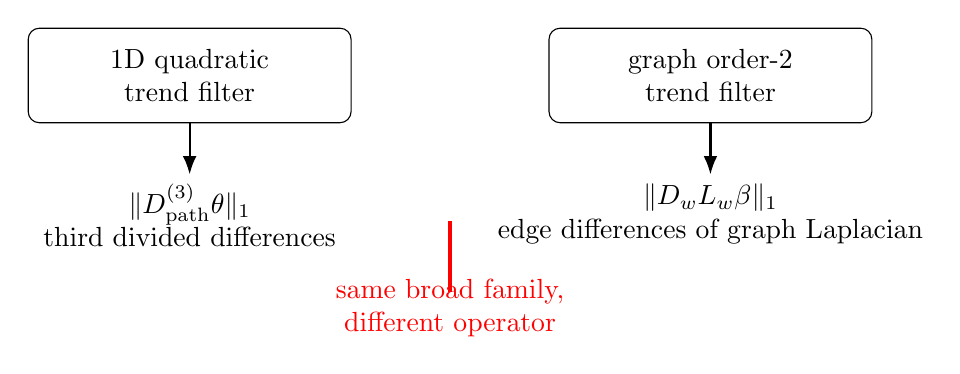
\begin{tikzpicture}[>=Latex,node distance=2.5cm]
  \node[draw,rounded corners,align=center,minimum width=4.1cm,minimum height=1.2cm] (oneD)
    {1D quadratic\\trend filter};
  \node[draw,rounded corners,align=center,minimum width=4.1cm,minimum height=1.2cm,right=of oneD] (graph)
    {graph order-2\\trend filter};
  \node[align=center,below=0.65cm of oneD] (oneDpen)
    {\(\|D^{(3)}_{\mathrm{path}}\theta\|_1\)\\third divided differences};
  \node[align=center,below=0.65cm of graph] (graphpen)
    {\(\|D_wL_w\beta\|_1\)\\edge differences of graph Laplacian};
  \draw[->,thick] (oneD) -- (oneDpen);
  \draw[->,thick] (graph) -- (graphpen);
  \draw[red,very thick] ($(oneD)!0.5!(graph)+(0,-1.85)$) -- ++(0,-0.9);
  \node[red,align=center] at ($(oneD)!0.5!(graph)+(0,-2.95)$)
    {same broad family,\\different operator};
\end{tikzpicture}
\caption{Both methods are \(\ell_1\)-adaptive smoothers, but they use different
penalty operators.  The penalty operator is the algorithmic heart of trend
filtering.}
\end{figure}

\section{What the 1D Quadratic Trend Filter Solves}

Assume we observe ordered samples
\[
  x_1 < x_2 < \cdots < x_n,
  \qquad y_i = f(x_i) + \varepsilon_i.
\]
The 1D trend filter estimates fitted values
\[
  \theta = (\theta_1,\ldots,\theta_n)^T,
  \qquad \theta_i \approx f(x_i).
\]

For order \(k=2\), \texttt{genlasso::trendfilter(y, pos = x, ord = 2)}
solves a generalized lasso problem of the form
\[
  \widehat\theta_\lambda
  =
  \argmin_{\theta\in\R^n}
  \left\{
    \frac{1}{2}\norm{y-\theta}_2^2
    +
    \lambda\norm{D^{(3)}_{\mathrm{pos}}\theta}_1
  \right\}.
\]
The matrix \(D^{(3)}_{\mathrm{pos}}\) computes third-order divided differences.
When the \(x_i\) are equally spaced, the interior stencil is
\[
  -\theta_i + 3\theta_{i+1} - 3\theta_{i+2} + \theta_{i+3}.
\]
The sign does not matter because the penalty takes absolute values.

\subsection{The Equal-Spaced Matrix}

For \(n=7\), the equal-spaced order-2 trend-filtering penalty matrix is
\[
D^{(3)}_{\mathrm{path}}
=
\begin{bmatrix}
-1 &  3 & -3 &  1 &  0 &  0 &  0\\
 0 & -1 &  3 & -3 &  1 &  0 &  0\\
 0 &  0 & -1 &  3 & -3 &  1 &  0\\
 0 &  0 &  0 & -1 &  3 & -3 &  1
\end{bmatrix}.
\]
There are \(n-3\) rows.  This is important: the penalty does not try to define
a third difference at the two boundaries.  It only penalizes the interior
third differences.

\subsection{What This Makes Unpenalized}

A third difference is zero for any quadratic sequence.  Therefore
\[
  D^{(3)}_{\mathrm{path}}\theta = 0
\]
whenever \(\theta_i\) lies on a quadratic curve in \(i\), or more generally
on a quadratic curve in \(x_i\) when divided differences are used.  The null
space has dimension \(3\):
\[
  \theta_i = a + b x_i + c x_i^2.
\]
This is the sense in which order-2 trend filtering is ``piecewise quadratic.''
Where the third differences are zero, the fitted curve behaves like a quadratic.
Where a third difference is nonzero, the method permits a knot, or local change
in curvature.

\begin{figure}[ht]
\centering
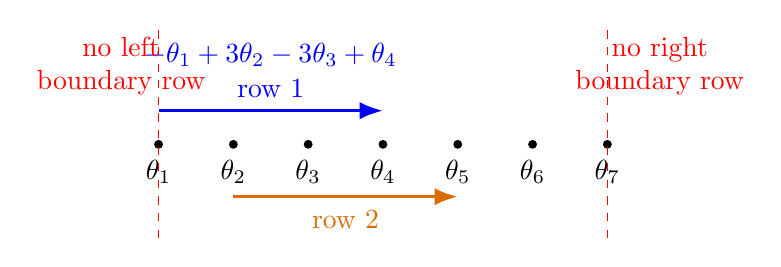
\begin{tikzpicture}[x=0.95cm,y=0.95cm,>=Latex]
  \foreach \i in {1,...,7} {
    \fill[black] (\i,0) circle (1.6pt);
    \node[below] at (\i,-0.08) {\(\theta_{\i}\)};
  }
  \draw[blue,very thick,->] (1,0.45) -- (4,0.45);
  \node[blue,above] at (2.5,0.50) {row 1};
  \node[blue,align=center] at (2.5,1.20)
    {\(-\theta_1+3\theta_2-3\theta_3+\theta_4\)};

  \draw[orange!85!black,very thick,->] (2,-0.70) -- (5,-0.70);
  \node[orange!85!black,below] at (3.5,-0.75) {row 2};

  \draw[red,dashed] (1,-1.25) -- (1,1.55);
  \draw[red,dashed] (7,-1.25) -- (7,1.55);
  \node[red,align=center] at (0.5,1.05) {no left\\boundary row};
  \node[red,align=center] at (7.7,1.05) {no right\\boundary row};
\end{tikzpicture}
\caption{The 1D order-2 trend filter penalizes sliding four-point third
differences.  It has no boundary third-difference rows, which helps preserve a
quadratic null space.}
\end{figure}

\section{What the Current Graph Order-2 Fit Solves}

The phase-2 \texttt{gflow} graph trend-filtering implementation follows the
graph operators
\[
  D_w,\qquad L_w = D_w^T D_w,\qquad \Delta_w^{(3)} = D_wL_w.
\]
For \texttt{order = 2}, the fit solves
\[
  \widehat\beta_\lambda
  =
  \argmin_{\beta\in\R^n}
  \left\{
    \frac{1}{2}\norm{y-\beta}_2^2
    +
    \lambda\norm{D_wL_w\beta}_1
  \right\}.
\]

Here \(D_w\) is a weighted oriented incidence matrix.  For an edge
\(e=(i,j)\),
\[
  (D_w\beta)_e = \omega_e(\beta_j-\beta_i).
\]
The weighted graph Laplacian is
\[
  L_w = D_w^TD_w.
\]
Thus \(L_w\beta\) is a graph-Laplacian signal on vertices, and \(D_wL_w\beta\)
computes edge differences of that Laplacian signal.

\subsection{What Happens on an Unweighted Path}

On an unweighted path with \(n=7\), the current graph order-2 penalty matrix is
\[
D L
=
\begin{bmatrix}
-2 &  3 & -1 &  0 &  0 &  0 &  0\\
 1 & -3 &  3 & -1 &  0 &  0 &  0\\
 0 &  1 & -3 &  3 & -1 &  0 &  0\\
 0 &  0 &  1 & -3 &  3 & -1 &  0\\
 0 &  0 &  0 &  1 & -3 &  3 & -1\\
 0 &  0 &  0 &  0 &  1 & -3 &  2
\end{bmatrix}.
\]
The middle rows look like third differences, up to sign.  But the first and
last rows are different:
\[
  -2\beta_1 + 3\beta_2 - \beta_3,
  \qquad
  \beta_5 - 3\beta_6 + 2\beta_7.
\]
These are boundary rows.  They are not present in the ordinary 1D quadratic
trend-filtering matrix.

Even more importantly, this matrix has \(n-1\) rows and rank \(n-1\) on a
connected path.  Its null space has dimension \(1\): constants only.  It does
not leave linear or quadratic trends unpenalized.

\begin{figure}[ht]
\centering
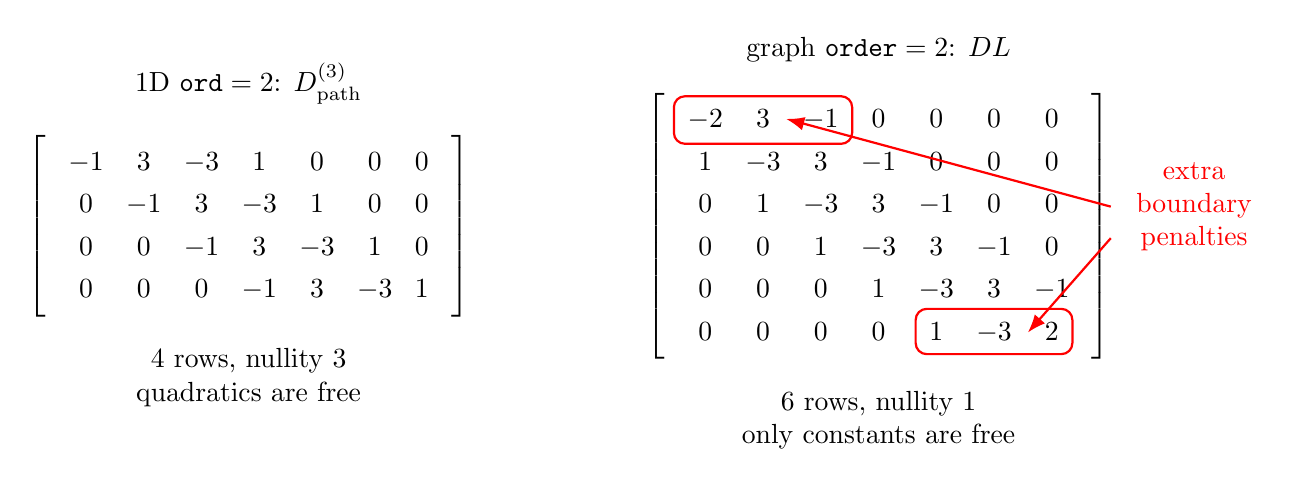
\begin{tikzpicture}[>=Latex]
  \matrix[matrix of math nodes,left delimiter={[},right delimiter={]},
          nodes={minimum width=0.36cm,minimum height=0.38cm},
          column sep=0.05cm,row sep=0.05cm] (A) at (0,0) {
    -1 &  3 & -3 &  1 &  0 &  0 &  0\\
     0 & -1 &  3 & -3 &  1 &  0 &  0\\
     0 &  0 & -1 &  3 & -3 &  1 &  0\\
     0 &  0 &  0 & -1 &  3 & -3 &  1\\
  };
  \node[above=0.25cm of A] {1D \(\texttt{ord}=2\): \(D^{(3)}_{\mathrm{path}}\)};
  \node[below=0.25cm of A,align=center] {4 rows, nullity 3\\quadratics are free};

  \matrix[matrix of math nodes,left delimiter={[},right delimiter={]},
          nodes={minimum width=0.36cm,minimum height=0.38cm},
          column sep=0.05cm,row sep=0.05cm] (B) at (8.0,0) {
    -2 &  3 & -1 &  0 &  0 &  0 &  0\\
     1 & -3 &  3 & -1 &  0 &  0 &  0\\
     0 &  1 & -3 &  3 & -1 &  0 &  0\\
     0 &  0 &  1 & -3 &  3 & -1 &  0\\
     0 &  0 &  0 &  1 & -3 &  3 & -1\\
     0 &  0 &  0 &  0 &  1 & -3 &  2\\
  };
  \node[above=0.25cm of B] {graph \(\texttt{order}=2\): \(DL\)};
  \node[below=0.25cm of B,align=center] {6 rows, nullity 1\\only constants are free};

  \draw[red,thick,rounded corners] ($(B-1-1.north west)+(-0.05,0.05)$)
    rectangle ($(B-1-3.south east)+(0.05,-0.05)$);
  \draw[red,thick,rounded corners] ($(B-6-5.north west)+(-0.05,0.05)$)
    rectangle ($(B-6-7.south east)+(0.05,-0.05)$);
  \node[red,align=center,anchor=west] at (11.15,0.25)
    {extra\\boundary\\penalties};
  \draw[red,->,thick] (10.95,0.25) -- ($(B-1-2.east)+(0.08,0)$);
  \draw[red,->,thick] (10.95,-0.15) -- ($(B-6-6.east)+(0.08,0)$);
\end{tikzpicture}
\caption{On a path, the current graph order-2 operator is not the same matrix
as the ordinary 1D order-2 trend-filtering operator.  The extra boundary rows
and smaller null space change the estimator.}
\end{figure}

\section{The Null Space Explains Much of the RMSE Gap}

The null space is the set of fitted signals that receive no roughness penalty.
It tells us what the smoother regards as globally simple.

\begin{center}
\begin{tabular}{lll}
\toprule
Method & Penalty matrix & Unpenalized signals\\
\midrule
1D \(\texttt{ord}=2\) trend filter & \(D^{(3)}_{\mathrm{path}}\) &
quadratic trends\\
current graph \(\texttt{order}=2\) & \(D_wL_w\) &
constants, for connected path\\
\bottomrule
\end{tabular}
\end{center}

This matters for Gaussian mixtures.  A Gaussian peak is smooth and curved.  A
piecewise quadratic estimator can approximate it with relatively few knots:
many intervals can behave like quadratic arcs.  The current graph order-2
operator does not grant the same freedom.  It still penalizes linear and
quadratic global behavior, especially through the boundary rows and through the
graph-Laplacian construction.

\begin{figure}[ht]
\centering
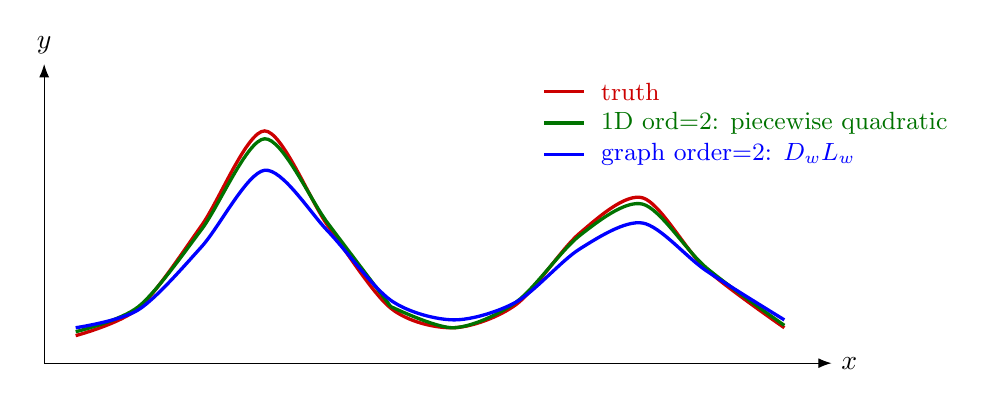
\begin{tikzpicture}[x=1cm,y=1cm,>=Latex]
  \draw[->] (0,0) -- (10,0) node[right] {\(x\)};
  \draw[->] (0,0) -- (0,3.8) node[above] {\(y\)};
  \draw[red!80!black,very thick,smooth]
    plot coordinates {(0.4,0.35) (1.2,0.70) (2.0,1.75) (2.8,2.95)
                      (3.6,1.75) (4.4,0.70) (5.2,0.45)
                      (6.0,0.75) (6.8,1.65) (7.6,2.10)
                      (8.4,1.20) (9.4,0.45)};
  \draw[green!45!black,very thick]
    plot[smooth] coordinates {(0.4,0.40) (1.2,0.72) (2.0,1.70)
                              (2.8,2.85) (3.6,1.78) (4.4,0.72)};
  \draw[green!45!black,very thick]
    plot[smooth] coordinates {(4.4,0.72) (5.2,0.45) (6.0,0.78)
                              (6.8,1.62) (7.6,2.02) (8.4,1.22) (9.4,0.48)};
  \draw[blue,very thick]
    plot[smooth] coordinates {(0.4,0.45) (1.2,0.68) (2.0,1.48)
                              (2.8,2.45) (3.6,1.68) (4.4,0.80)
                              (5.2,0.55) (6.0,0.78) (6.8,1.45)
                              (7.6,1.78) (8.4,1.18) (9.4,0.55)};
  \draw[red!80!black,very thick] (6.35,3.45) -- (6.85,3.45);
  \node[red!80!black,anchor=west,font=\small] at (6.95,3.45) {truth};
  \draw[green!45!black,very thick] (6.35,3.05) -- (6.85,3.05);
  \node[green!45!black,anchor=west,font=\small] at (6.95,3.05)
    {1D ord=2: piecewise quadratic};
  \draw[blue,very thick] (6.35,2.65) -- (6.85,2.65);
  \node[blue,anchor=west,font=\small] at (6.95,2.65)
    {graph order=2: \(D_wL_w\)};
\end{tikzpicture}
\caption{A Gaussian-mixture signal is smooth and curved.  A 1D quadratic trend
filter has exactly the right low-order local model: quadratic arcs separated by
adaptive knots.}
\end{figure}

\section{The Operators Also Handle Unequal Spacing Differently}

The benchmark samples \(x_i\) randomly in \([0,1]\), so the path spacing is not
constant.  The 1D trend filter uses \texttt{pos = x}.  This means the penalty
matrix is a divided-difference operator that accounts for unequal spacing:
\[
  D^{(3)}_{\mathrm{pos}} = D^{(3)}(x_1,\ldots,x_n).
\]
Two gaps of different length are not treated as identical.

The current graph trend-filtering implementation receives only an adjacency
list and edge weights.  In the subset benchmark, the unit graph variant ignores
spacing entirely, while the metric-weighted variants transform edge lengths
into conductance-like weights.  That is not the same as divided differences.

Divided differences approximate derivatives with respect to \(x\).  Conductance
weights express how strongly adjacent vertices should be fused or smoothed.
Both use edge lengths, but they encode different mathematical meanings.

\begin{figure}[ht]
\centering
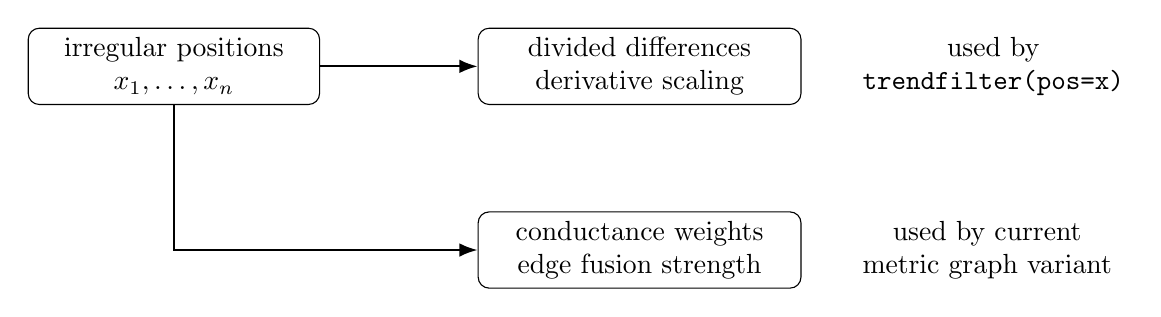
\begin{tikzpicture}[>=Latex,node distance=2.0cm]
  \node[draw,rounded corners,align=center,minimum width=3.7cm] (x)
    {irregular positions\\\(x_1,\ldots,x_n\)};
  \node[draw,rounded corners,align=center,minimum width=4.1cm,right=of x] (div)
    {divided differences\\derivative scaling};
  \node[draw,rounded corners,align=center,minimum width=4.1cm,below=1.35cm of div] (cond)
    {conductance weights\\edge fusion strength};
  \draw[->,thick] (x) -- (div);
  \draw[->,thick] (x) |- (cond);
  \node[align=center,right=0.65cm of div] {used by\\\texttt{trendfilter(pos=x)}};
  \node[align=center,right=0.65cm of cond] {used by current\\metric graph variant};
\end{tikzpicture}
\caption{The specialized 1D trend filter and the graph metric-weighted variant
both see the sample spacing, but they use it differently.}
\end{figure}

\section{The Cross-Validation Procedures Differ Too}

There is another important difference.  The baseline uses
\[
  \texttt{genlasso::cv.trendfilter(fit,\ mode = "lambda")}.
\]
That routine is specialized for one-dimensional trend filtering.  When it holds
out interior points, it predicts them by interpolation from neighboring
training positions.  This matches the ordered 1D regression problem.

The current \texttt{fit.graph.trend.filtering()} cross-validation is graph
generic.  It forms a training selection matrix \(X\), fits the generalized
lasso to the observed vertices, and reads predictions for held-out vertices
from the full coefficient vector.  That is a reasonable generic graph CV
strategy, but it is not the same criterion as \texttt{cv.trendfilter()}.

Thus even if the penalty matrix were made identical, the selected \(\lambda\)
could still differ unless the CV procedure were also made identical.

\section{Why the Benchmark Gap Is Expected}

The gap
\[
  0.0322 \quad\text{versus}\quad 0.0252
\]
is not mysterious once the operators are laid side by side.

\begin{enumerate}
  \item The 1D baseline uses the exact order-2 path divided-difference
        operator.
  \item That operator has a quadratic null space, which is well matched to
        smooth Gaussian peaks.
  \item The current graph order-2 operator \(D_wL_w\) does not have the same
        null space on a path; it leaves only constants unpenalized.
  \item The current graph operator adds boundary penalties absent from the 1D
        trend-filtering matrix.
  \item The graph metric-weighted variants use conductance weights, not the
        divided-difference scaling used by \texttt{trendfilter(pos=x)}.
  \item The CV procedures select \(\lambda\) by different prediction rules.
\end{enumerate}

\begin{figure}[ht]
\centering
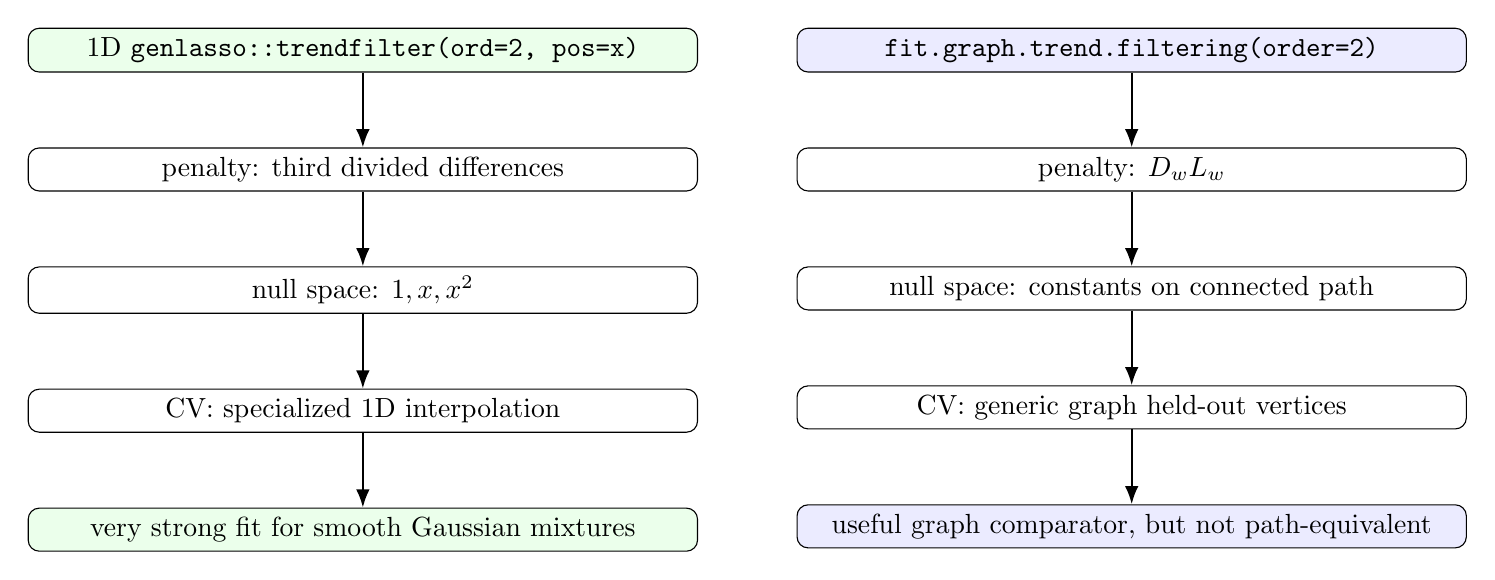
\begin{tikzpicture}[>=Latex,node distance=0.95cm]
  \node[draw,rounded corners,align=center,fill=green!8,minimum width=8.5cm] (a)
    {1D \texttt{genlasso::trendfilter(ord=2, pos=x)}};
  \node[draw,rounded corners,align=center,below=of a,minimum width=8.5cm] (b)
    {penalty: third divided differences};
  \node[draw,rounded corners,align=center,below=of b,minimum width=8.5cm] (c)
    {null space: \(1,x,x^2\)};
  \node[draw,rounded corners,align=center,below=of c,minimum width=8.5cm] (d)
    {CV: specialized 1D interpolation};
  \node[draw,rounded corners,align=center,below=of d,fill=green!8,minimum width=8.5cm] (e)
    {very strong fit for smooth Gaussian mixtures};

  \node[draw,rounded corners,align=center,fill=blue!8,minimum width=8.5cm,right=1.25cm of a] (aa)
    {\texttt{fit.graph.trend.filtering(order=2)}};
  \node[draw,rounded corners,align=center,below=of aa,minimum width=8.5cm] (bb)
    {penalty: \(D_wL_w\)};
  \node[draw,rounded corners,align=center,below=of bb,minimum width=8.5cm] (cc)
    {null space: constants on connected path};
  \node[draw,rounded corners,align=center,below=of cc,minimum width=8.5cm] (dd)
    {CV: generic graph held-out vertices};
  \node[draw,rounded corners,align=center,below=of dd,fill=blue!8,minimum width=8.5cm] (ee)
    {useful graph comparator, but not path-equivalent};

  \foreach \u/\v in {a/b,b/c,c/d,d/e,aa/bb,bb/cc,cc/dd,dd/ee}
    \draw[->,thick] (\u) -- (\v);
\end{tikzpicture}
\caption{The two methods differ at several algorithmic layers: penalty,
unpenalized space, spacing semantics, and cross-validation.}
\end{figure}

\section{How to Make the 1D Case Match Exactly}

If the goal is for \texttt{gflow} to reproduce the 1D trend-filtering
algorithm on path graphs, then \texttt{fit.graph.trend.filtering(order = 2)}
should not use \(D_wL_w\) in that mode.  It should use the same path
divided-difference matrix as \texttt{genlasso::trendfilter()}.

\subsection{Add a Path-Compatible Operator Family}

One clean API direction is to separate the operator family from the order:
\[
\texttt{operator.family}
\in
\{\texttt{"graph.laplacian"},\ \texttt{"path.divided.difference"}\}.
\]
Then:
\[
\begin{array}{lll}
\texttt{operator.family = "graph.laplacian"}:
& k=0:D_w,\quad k=1:L_w,\quad k=2:D_wL_w,\\[3pt]
\texttt{operator.family = "path.divided.difference"}:
& k=0:D^{(1)}_{\mathrm{pos}},\quad
  k=1:D^{(2)}_{\mathrm{pos}},\quad
  k=2:D^{(3)}_{\mathrm{pos}}.
\end{array}
\]

For a path graph, \(\texttt{pos}\) can be supplied directly, or reconstructed
from metric edge lengths when the graph is a single path with two endpoints.
For exact reproduction of \texttt{genlasso::trendfilter()}, the safest API is
to require explicit vertex positions:
\[
  \texttt{vertex.position = x}.
\]

\subsection{Use the Same Solver and Lambda Selection}

To reproduce the benchmark baseline exactly, matching the penalty matrix is not
enough.  The implementation should also call the same trend-filtering path and
CV routines:
\[
  \texttt{genlasso::trendfilter(y,\ pos = x,\ ord = 2)}
\]
and
\[
  \texttt{genlasso::cv.trendfilter(...,\ mode = "lambda")}.
\]

That suggests a second API switch:
\[
  \texttt{lambda.selection = "path.cv"}
\]
or perhaps
\[
  \texttt{solver = "genlasso.trendfilter"}
\]
for path-compatible fits.  With the same \(y\), the same \(x\), the same
operator, and the same CV rule, \texttt{gflow} should be able to match the
1D baseline's fitted values and RMSE up to numerical tolerance.

\section{How to Keep the Graph Method Honest}

The graph-Laplacian operator \(D_wL_w\) is still scientifically meaningful.  It
is a real graph trend-filtering operator in the graph literature's sense.  It
asks for sparsity in edge differences of graph Laplacian values.  That is a
reasonable graph analogue when there is no global ordering and no notion of a
polynomial in \(x\).

But it should be presented as a graph method, not as a drop-in replacement for
1D trend filtering.  In benchmark reports, the distinction should be explicit:

\begin{center}
\begin{tabular}{p{0.36\linewidth}p{0.52\linewidth}}
\toprule
Question & Recommended operator\\
\midrule
Do we want exact 1D trend-filtering behavior on a path? &
Use path divided differences \(D^{(k+1)}_{\mathrm{pos}}\).\\
Do we want a graph-native Wang-style operator on an arbitrary graph? &
Use incidence/Laplacian operators \(D_w\), \(L_w\), \(D_wL_w\).\\
Do we want metric graph trend filtering? &
Decide explicitly how metric lengths become \(\omega_e\), and do not assume
this equals divided differences.\\
\bottomrule
\end{tabular}
\end{center}

\section{Recommended \texttt{gflow} Modifications}

Here is the most direct path to make the 1D case match the benchmark winner.

\begin{enumerate}
  \item Add a path-divided-difference operator constructor, possibly
        \[
          \texttt{path.trend.filtering.operator(x,\ order)}.
        \]
        It should return the exact \(D^{(k+1)}_{\mathrm{pos}}\) matrix used by
        \texttt{genlasso}.

  \item Add a mode to \texttt{fit.graph.trend.filtering()}:
        \[
          \texttt{operator.family = c("graph.laplacian", "path.divided.difference")}.
        \]
        The default can remain graph-native for arbitrary graphs.

  \item For \texttt{operator.family = "path.divided.difference"}, require
        \texttt{vertex.position} or reconstruct it only when the graph is
        provably a single path.

  \item Add \texttt{lambda.selection = "path.cv"} or a solver option that uses
        \texttt{genlasso::cv.trendfilter()} instead of generic graph CV.

  \item Add tests asserting exact agreement with
        \texttt{genlasso::trendfilter(y, pos = x, ord = order)} for
        \(\texttt{order}=0,1,2\) on small path graphs.

  \item Keep \(D_wL_w\) as the graph-native order-2 operator, and document that
        it is not path-equivalent to ordinary quadratic trend filtering.
\end{enumerate}

\section{Summary}

The RMSE difference \(0.0322\) versus \(0.0252\) is not mainly a tuning
accident.  The two estimators use different penalty matrices.  The specialized
1D quadratic trend filter has the right null space and spacing semantics for
smooth one-dimensional Gaussian-mixture regression.  The current graph order-2
fit is a graph-native Laplacian-difference estimator; on a path, it is close in
spirit but not algebraically equivalent.

To get the same algorithm and therefore the same 1D RMSE behavior, \texttt{gflow}
should add a path-divided-difference operator family and, when exact parity is
desired, reuse the same \texttt{genlasso::trendfilter()} and
\texttt{cv.trendfilter()} machinery.  That would let \texttt{gflow} offer both:
an exact 1D trend-filtering compatibility mode for path graphs, and a
graph-native trend-filtering mode for arbitrary weighted graphs.

\end{document}
